\documentclass[11pt]{article}
\usepackage[utf8]{inputenc}
\usepackage[T1]{fontenc}
\usepackage{graphicx}
\usepackage{grffile}
\usepackage{longtable}
\usepackage{wrapfig}
\usepackage{rotating}
\usepackage[normalem]{ulem}
\usepackage{amsmath}
\usepackage{textcomp}
\usepackage{amssymb}
\usepackage{capt-of}
\usepackage{hyperref}
\usepackage{minted}
\usepackage[edges]{forest}

\usetikzlibrary{arrows.meta}
\widowpenalties 1 10000
\raggedbottom
\sloppy

\usepackage{hyperref}
\hypersetup{colorlinks, linkcolor={red!50!black}, citecolor={blue!50!black}, urlcolor={blue!80!black}}

\usepackage[nottoc,notlot,notlof]{tocbibind}

\usepackage{caption} 
\captionsetup[table]{skip=8pt}

% https://aty.sdsu.edu/bibliog/latex/floats.html
% Alter some LaTeX defaults for better treatment of figures:
    % See p.105 of "TeX Unbound" for suggested values.
    % See pp. 199-200 of Lamport's "LaTeX" book for details.
    %   General parameters, for ALL pages:
    \renewcommand{\topfraction}{0.9}  % max fraction of floats at top
    \renewcommand{\bottomfraction}{0.8} % max fraction of floats at bottom
    %   Parameters for TEXT pages (not float pages):
    \setcounter{topnumber}{2}
    \setcounter{bottomnumber}{2}
    \setcounter{totalnumber}{4}     % 2 may work better
    \renewcommand{\dbltopfraction}{0.9} % fit big float above 2-col. text
    \renewcommand{\textfraction}{0.07}  % allow minimal text w. figs
    %   Parameters for FLOAT pages (not text pages):
    \renewcommand{\floatpagefraction}{0.7}  % require fuller float pages
  % N.B.: floatpagefraction MUST be less than topfraction !!
    \renewcommand{\dblfloatpagefraction}{0.7} % require fuller float pages

  % remember to use [htp] or [htpb] for placement

% https://tex.stackexchange.com/questions/70202/expand-placeins-functonality-to-subsections
\usepackage[section]{placeins}
\makeatletter
\AtBeginDocument{%
     \expandafter\renewcommand\expandafter\subsection\expandafter
       {\expandafter\@fb@subsecFB\subsection}%
     \newcommand\@fb@subsecFB{\FloatBarrier
     \gdef\@fb@afterHHook{\@fb@topbarrier \gdef\@fb@afterHHook{}}}
     \g@addto@macro\@afterheading{\@fb@afterHHook}
     \gdef\@fb@afterHHook{}
  }
\AtBeginDocument{%
     \expandafter\renewcommand\expandafter\subsubsection\expandafter
       {\expandafter\@fb@subsubsecFB\subsubsection}%
     \newcommand\@fb@subsubsecFB{\FloatBarrier
     \gdef\@fb@afterHHook{\@fb@topbarrier \gdef\@fb@afterHHook{}}}
     \g@addto@macro\@afterheading{\@fb@afterHHook}
     \gdef\@fb@afterHHook{}
  }
\makeatother

\setminted{frame=lines}
\AtEndEnvironment{listing}{\vspace{-8pt}}

\usepackage{array}
\usepackage{csquotes}
\usepackage{multirow}
\usepackage{graphicx}
\usepackage{adjustbox}
\author{Matthew Barber}
\date{\today}
\title{Testing a Randomness Testing Suite}
\hypersetup{
 pdfauthor={Matthew Barber},
 pdftitle={Testing a Randomness Testing Suite},
 pdfkeywords={},
 pdfsubject={},
 pdfcreator={Emacs 26.3 (Org mode 9.3.6)}, 
 pdflang={English}
}
\begin{document}

\maketitle
\vspace*{\fill}

\begin{center}
  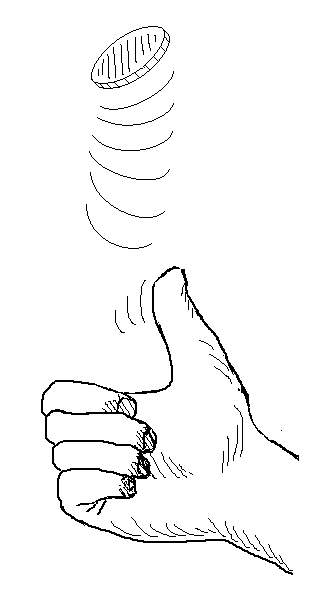
\includegraphics[height=.5\linewidth]{./toss.png}
\end{center}

\begin{abstract}
\textit{coinflip} is a Python library for randomness testing, which also includes a command-line interface. This paper discusses how coinflip itself is tested.

After the introduction, the following sections detail the strategies used in testing coinflip's own randomness tests and its CLI. A final evaluation is found at the end, with a bibliography and appendix items following suit.
  
Note the term \textit{SP800-22} is the publication code of the paper by NIST which specifies the randomness tests that coinflip implements \cite{nist}. The code is used as a shorthand due to it being deeply referenced.
  
  Word count: 2458 (body text + captions)
\end{abstract}
\newpage
\tableofcontents
\newpage

\section{Introduction}
\label{sec:org0e0f4cc}
coinflip uses the \textit{pytest} \cite{pytest} package to test coinflip's own randomness tests, as well as its CLI. It also incorporates the \emph{Hypothesis} \cite{hypothesis} library, which provides various tools for property-based and model-based testing.

This report deviates from the recommended structure of per-quadrant sections as per the agile quadrants, due to the various unconventional testing strategies employed which acted in multiple quadrant domains to uncover bugs/problems in those multiple quadrants. The quadrants were only used to assess iterations of coinflip's overall testing strategy---not as a top-down tool to devise a plan beforehand.

\begin{table}[H]
  \caption{The agile quadrants covered by the sections in this report.}
\begin{adjustbox}{center}
  \begin{tabular}%
    {
    >{\raggedleft\arraybackslash}p{0.5cm}%
    >{\raggedright\arraybackslash}p{5cm}%
    >{\raggedleft\arraybackslash}p{5cm}%
    >{\raggedright\arraybackslash}p{0.5cm}%
    }
    \multicolumn{4}{c}{\small{Business facing}} \\
    \multirow{11}{*}{\rotatebox{90}{\small{Support team}}} & \textbf{Q2} & \textbf{Q3} & \multirow{9}{*}{\rotatebox{270}{\small{Critique product}}}  \\
    \multirow{11}{*}{} & \ref{sec:examples} Known test cases & \ref{sec:compare} Suite comparisons & \multirow{9}{*}{} \\
    \multirow{11}{*}{} & \ref{sec:model} Stateful CLI & \ref{sec:model} Stateful CLI & \multirow{9}{*}{}\\
    & & & \\
    & & & \\
    \noalign{\bigskip}
    \multirow{11}{*}{} &  &  \ref{sec:smoke} Successful exits & \multirow{9}{*}{}\\
    \multirow{11}{*}{} &  &  \ref{sec:property} Generating tests & \multirow{9}{*}{}\\
    \multirow{11}{*}{} &  & \ref{sec:model} Stateful CLI & \multirow{9}{*}{}\\
    \multirow{11}{*}{} & \ref{sec:compare} Suite comparisons  & \ref{sec:ci} Tooling & \multirow{9}{*}{}\\
    \multirow{11}{*}{} & \textbf{Q1} & \textbf{Q4} & \multirow{9}{*}{}\\
    \multicolumn{4}{c}{\small{Technology facing}}\\
  \end{tabular}
\end{adjustbox}
\end{table}

\section{Testing the randomness tests}

Randomness tests are hypothesis tests, identifying some property of a sample output from the RNG represented in a \emph{test statistic}, which is compared to a hypothetically truly random sequence. A \emph{p-value} results from these tests, suggesting the probability that a truly random sequence would have the characteristics of the RNG output---the lower the p-value, the less confident one can say the RNG is truly random.

The NIST paper \textit{Statistical test suite for random and pseudorandom number generators for cryptographic applications} \cite{nist} describes the randomness tests that coinflip implements. These tests take sampled RNG output, which would be a binary sequence. The paper will be referred to as it's internal publication code \emph{SP800-22}.

\begin{listing}
\begin{minted}[]{pycon}
>>> from coinflip.randtests import monobits
>>> help(monobits)
monobits(sequence):
    Proportion of values is compared to expected 1:1 ratio

    The difference between the frequency of the two values is found, and
    referenced to a hypothetically truly random RNG.

    Parameters
    ----------
    sequence : array-like
        Output of the RNG being tested

    Returns
    -------
    MonobitsTestResult
        Dataclass that contains the test's statistic and p-value as well as
        other relevant information gathered.
>>> from random import getrandbits
>>> sample_RNG_output = [getrandbits(1) for _ in range(5)]
>>> print(sample_RNG_output)
[0, 1, 0, 0, 1]
>>> result = monobits(sample_RNG_output)
>>> print(result)
normalised diff  0.447
p-value          0.655

value      count
-------  -------
0              3
1              2
\end{minted}
\caption{Example usage of the \textit{Monobits} randomness test in coinflip.}
\end{listing}

\subsection[Known test cases]{Known test cases\\ \small{Covers: \emph{white-box, story}}}
\label{sec:examples}

SP800-22 includes worked examples for their recommend randomness tests, which was used to help verify the implemented tests. The results of these examples are asserted to the results of coinflip's own implementations under the same parameters.


\begin{listing}[htbp]
\begin{minted}[]{python}
from coinflip.randtests import monobits
...
def test_monobits():
    bits = [1, 0, 1, 1, 0, 1, 0, 1, 0, 1]

    result = monobits(bits)

    assert isclose(result.statistic, 0.632455532)
    assert isclose(result.p, 0.527089)
\end{minted}
\caption{\label{code:test_monobits}Original pytest method to test the \emph{Monobits} randomness test. \texttt{bits} is passed as the \texttt{sequence} argument to the \texttt{monobits} method, and a \texttt{result} is captured and compared to the expected statistic and p-value.}
\end{listing}

\begin{figure}[htbp]
  \begin{enumerate}
    \item The zeros and ones of the input sequence ($\epsilon$) are converted to values of –1 and +1 and are added together to produce $S_n = X_1 + X_2 + ... + X_n$, where $X_i = 2\epsilon{}_i - 1$.
    
    e.g. if $\epsilon = 1011010101$, then $n = 10$ and $S_n = 1 + (-1) + 1 + 1 + (-1) + 1 + (-1) + 1 + (-1) + 1 = 2$.
    
    \item Compute the test statistic $S_{obs} = \left| S_n \right| / \sqrt{n}$
    
    e.g. in this section, $S_{obs} = \left| 2 \right| / \sqrt{10} = 0.632455532$.
    
    \item Compute $p = erfc(S_{obs} / \sqrt{2})$, where $erfc$ is the complementary error function.
    
    e.g. $p = erfc(0.6324555 / \sqrt{2}) = 0.527089$.
  \end{enumerate}
  \caption{Walkthrough the \textit{Monobits} test with a concrete example, provided by SP800-22.}
\end{figure}


Additionally, the working out provided in SP800-22 helped in debugging the tests, as the walkthroughs could be reviewed step-by-step by use of a debugger (i.e. the Python debugger \texttt{pdb}) to see where exactly miscalculation occurred.

As the number of test methods such as in listing \ref{code:test_monobits} grew,
the code became confusing to navigate which frustrated debugging. As all the
examples followed a similar pattern, a container \texttt{Example} was made to specify the parameters of  tests programmatically.

\begin{listing}[htbp]
\begin{minted}[]{python}
class Example(NamedTuple):
    randtest: str
    bits: List[int]
    statistic: Union[int, float]
    p: float
    kwargs: Dict[str, Any] = {}
\end{minted}
\caption[\texttt{Example} definition]{The named tuple \texttt{Example}, which allows specification of SP800-22 examples.}
\end{listing}

\begin{listing}[htbp]
\begin{minted}[]{python}
examples = [
    Example(
        randtest="monobits",

        bits=[1, 0, 1, 1, 0, 1, 0, 1, 0, 1],

        statistic=.632455532,
        p=0.527089,
    ),
    ...
]
\end{minted}
\caption{List of SP800-22 examples to be paramtrised by pytest, specified as \texttt{Example} tuples.}
\end{listing}

We could specify fixtures for Gherkin text files, but the use of keywords to specify the \textit{given} (\texttt{randtest}), \textit{when} (\texttt{bits}, \texttt{kwargs}), and \textit{then} (\texttt{statistic}, \texttt{p}) of examples makes it easy enough to onboard non-technical users to write new test cases in the future.

\subsection[Generating test cases]{Generating test cases\\ \small{Covers: \emph{property-based, exploratory, performance, reliability}}}
\label{sec:property}

Property-based testing is employed to specify \emph{all} possible input for the randomness tests. This means generating data that meets the input specification at various extremes, which the Hypothesis library provides for.

Below is an explanation of how property-based testing works in Hypothesis, taken from their documentation \cite{hypothesis}.
\begin{displayquote}
Think of a normal unit test as being something like the following:

\begin{enumerate}
\item Set up some data.
\item Perform some operations on the data.
\item Assert something about the result.
\end{enumerate}

Hypothesis lets you write tests which instead look like this:

\begin{enumerate}
\item For all data matching some specification.
\item Perform some operations on the data.
\item Assert something about the result.
\end{enumerate}
\end{displayquote}

The input for all randomness tests will always include a binary sequences (the RNG output being tested), which can be declared as a Hypothesis \emph{strategy}. Strategies are data generators for property-based testing, i.e. generates data matching some specification.

A custom strategy \texttt{mixedbits()} was created to generate binary sequences in a seemingly randomised fashion. A small sample of generated sequences is available in appendix \ref{sec:sequences}.

Hypothesis will give "health check" errors when individual test cases take too long, i.e. if it's been more than 200 milliseconds for a test to end. It also purposely repeats sequences which were successful, to uncover any bugs which relate to global states.

\begin{listing}[htbp]
\begin{minted}[]{python}
from hypothesis import given
from hypothesis import strategies as st
...
def mixedbits():
    binary = st.integers(min_value=0, max_value=1)  # 0 or 1
    bits = st.lists(binary, min_size=2)
    mixedbits = bits.filter(contains_multiple_values)

    return mixedbits
...
@given(mixedbits())
def test_monobits(bits):
    result = randtests.monobits(bits)
    ...
\end{minted}
\caption[\texttt{mixedbits()} definition and usage]{\label{code:mixedbits}Declaration of the \texttt{mixedbits()} strategy and an example of it's use on the \emph{Monobits} randomness test. \texttt{contains\_multiple\_values()} is a filter for whether the sequence is multi-valued or not.}
\end{listing}
\FloatBarrier

Just running supposedly valid data on the implemented randomness tests and testing there are no warnings is very useful. For example, a bug was discovered in the \emph{Discrete Fourier Transform} test by using the \texttt{mixedbits()} strategy. The test only uses an even-lengthed sequence and will truncate any odd bits---this means it can be passed a valid binary sequence, but after truncation the sequence becomes single-valued, and so unexpectedly breaks the Fourier transform involved in the test. This unique scenario was discovered thanks to the generated boundary case, and now means users are raised a specific \texttt{NonBinaryTruncatedSequenceError} which explains the circumstance why the randomness test cannot accept their input.

\begin{listing}[htbp]
  \begin{minted}[]{pycon}
>>> from coinflip.randtests import discrete_fourier_transform
>>> discrete_fourier_transform([0, 0, 0, 0, 0, 0])
Traceback...
...NonBinarySequenceError: \
Sequence does not contain only 2 distinct values (i.e. binary)
>>> discrete_fourier_transform([0, 0, 0, 0, 0, 1])
Traceback...
...NonBinaryTruncatedSequenceError: \
When truncated into an even-length, sequence contains only 1 distinct value
i.e. the sequence was originally binary, but now isn't
  \end{minted}
  \caption[Interactive session showcasing \texttt{NonBinaryTruncatedSequenceError}]{The \texttt{NonBinarySequenceError} and derivative \texttt{NonBinaryTruncatedSequenceError} being raised when using the \emph{Discrete Fourier Transform} randomness test.}
\end{listing}

\subsection[Comparing to other suites]{Comparing to other suites\\ \small{Covers: \emph{boundary, equivalence, comparison, exploratory}}}
\label{sec:compare}

The results of the randomness tests using generated input can be compared to other implementations. Currently two open source Python programs are used, one by David Johnston \cite{dj}, and the other by Stuart Gordon Reid \cite{sgr}. 

Adapting these suites to mirror coinflip's own API enabled running the SP800-22 examples on them (section \ref{sec:examples}). If SP800-22's examples were taken as completely accurate, then it could lead to false-positives if it does infact have mistakes. When coinflip fails to match an example's conclusion, the other suites can be checked first to see if they reach they fail as well.

For example, a SP800-22 example for the \emph{Discrete Fourier Transform} test was failing in my own randomness test, however the Johnston and Reid implementations both got nearly the same result as myself. This helped identify a problem in the same SciPy \cite{scipy} fast Fourier transform method we were all using.

\begin{table}[htbp]
  \caption[p-values of \emph{Discrete Fourier Transform} implementations]{The p-values of the \emph{Discrete Fourier Transform} test for the same input sequence of \texttt{1001010011}.}
  \centering
  \begin{tabular}{lr}
    Implementation & p-value\\
    \hline
    SP800-22 & 0.029523\\
    coinflip & 0.468159\\
    Johnston & 0.468159\\
    Reid & 0.468159\\
  \end{tabular}
\end{table}

\FloatBarrier

Subsequently, we can compare the results of coinflip's randomness tests to the implementations from the same Hypothesis-generated inputs (section \ref{sec:property}).

Hypothesis generates sequences with numerous rubrics, including purposely generating boundary cases, and purposely generating cases that fit into automatically identified equivalence partitions (e.g. classes "sequence length" and "\texttt{0}-to-\texttt{1} ratios"). By comparing the results of other suites, we can verify all these cases are actually handled correctly.

A simple Hypothesis test method is for the \emph{Monobits} test, which has no keyword arguments and so should be determined by just the inputted sequence. This means a test method comparing different implementations only needs to be passed the sequences generated from the \texttt{mixedbits()} strategy shown in listing \ref{code:mixedbits}, and then assert the results of the implementations are similar enough to my randomness tests.

\begin{listing}[htbp]
\begin{minted}[]{python}
from .implementations import sgr
from .implementations import dj
...
@given(mixedbits())
def test_monobits(bits):
    result = randtests.monobits(pd.Series(bits))

    dj_result = dj.monobits(bits)
    assert isclose(result.p, dj_result.p)

    sgr_p = sgr.monobits(bits)
    assert isclose(result.p, sgr_p)
\end{minted}
\caption[Comparing coinflip's \emph{Monobits} implementation to others]{Simple comparison of Johnston's and Reid's implementation of the \emph{Monobits} test to my own, using generated sequences from the \texttt{mixedbits()} strategy.}
\end{listing}

Comparing results of different implementations gives further confidence on the accuracy and robustness of my randomness tests. In the future all open source test suites available should be adapted; a possible metric for accuracy for a specific randomness test in coinflip could be if it gets roughly the same p-values as the majority of the other test suites.

\section{Testing the command-line interface}

coinflip's CLI consists of subcommands to the \texttt{coinflip} group command. The subcommands provide various features to aid users in loading their RNG output samples and subsequently running the randomness tests on respective samples.


\begin{listing}[htbp]
  \begin{minted}[]{console}
$ coinflip --help
Usage: coinflip [OPTIONS] COMMAND [ARGS]...

Randomness tests for RNG output.

Output of random number generators can be parsed and serialised into a
test-ready format via the load command. The data is saved in a folder,
which coinflip refers to as a "store". This store is located in the local
data directory, but can be easily accessed via the store's name in coinflip
commands.

...

Options:
-h, ----help  Show this message and exit.

Commands:
example-run  Run randomness tests on example data.
load         Loads DATA into a store.
run          Run randomness tests on data in STORE.
ls           List all stores.
rm           Delete STORE.
...
  \end{minted}
  \caption[\texttt{conflip} command description]{Simplified description of the \texttt{coinflip} command.}
\end{listing}

\subsection[Successful exits]{Successful exit codes\\ \small{Covers: \emph{smoke}}}
\label{sec:smoke}

coinflip's command-line interface uses the Click \cite{click} package, which offers a mockable command-line interface via its \texttt{CliRunner} to conveniently run CLI commands. A simple smoke test is to execute commands and assert that their exit code is \texttt{0}, i.e. the command executed successfully without any errors. The \texttt{coinflip example-run} command is especially useful, in that it runs all the randomness tests and so covers more functionality.

\begin{listing}[htbp]
  \begin{minted}[]{console}
$ coinflip example-run --help
Usage: coinflip example-run [OPTIONS]

Run randomness tests on example data.
  \end{minted}
  \caption{Simplified description of the \texttt{coinflip example-run} command.}
\end{listing}

\begin{listing}[htbp]
\begin{minted}{python}
from click.testing import CliRunner
from coinflip import cli
...
def test_main():
    runner = CliRunner()
    result = runner.invoke(cli.main, [])

    assert result.exit_code == 0

def test_example_run():
    runner = CliRunner()
    result = runner.invoke(cli.example_run, [])

    assert result.exit_code == 0
\end{minted}
\caption[Smoke testing the coinflip CLI]{Simple smoke tests for the \texttt{coinflip} and \texttt{coinflip example-run} commands.}
\end{listing}

\subsection[Stateful testing]{Stateful testing\\ \small{Covers: \emph{model-based, functional, exploratory, reliability}}}
\label{sec:model}

coinflip's CLI allows users to load their data into \textit{stores}, where each store pertains to a specific RNG output sample. In actuality, the stores are simply folders which are located in the user's OS-specific user data directory (e.g. \texttt{\%AppData\%} in Windows); coinflip is providing an abstraction to these folders.

One can load their RNG output sample via the \texttt{coinflip load} command; can view the stores currently in their user data directory via the \texttt{coinflip ls} command; and can remove stores via the \texttt{command rm} command.

\begin{listing}[htbp]
  \begin{minted}[]{console}
$ coinflip ls
$ coinflip load rng_output_sample.txt
Store name to be encoded as store_20200721T093641Z
Data stored successfully!
...
$ coinflip ls
store_20200721T093641Z
$ coinflip rm store_20200721T093641Z
$ coinflip ls
  \end{minted}
  \caption[\texttt{conflip ls} command before and after \texttt{conflip load}]{Using the \texttt{coinflip ls} command, there are initially no stores. Loading RNG output via the \texttt{coinflip load} command, the subsequent call of \texttt{coinflip ls} shows that there is now a store of the aforementioned RNG output.}
\end{listing}

\begin{listing}[htbp]
  \begin{minted}[]{console}
$ ls $HOME/.local/share/coinflip
$ coinflip load rng_output_sample.txt
Store name to be encoded as store_20200721T093641Z
Data stored successfully!
...
$ ls $HOME/.local/share/coinflip
store_20200721T093641Z
$ coinflip rm store_20200721T093641Z
$ ls $HOME/.local/share/coinflip
  \end{minted}
  \caption[\texttt{ls} command before and after \texttt{conflip load}]{Using GNU's \texttt{ls} command on coinflip's user data directory on Ubuntu, there are initially no folders representing stores. Loading RNG output via the \texttt{coinflip load} command, the subsequent call of \texttt{ls} shows that there is now a folder representing a store.}
\end{listing}

To test these abstraction are robust, model-based testing was employed. Hypothesis has mechanisms that can allow specification of a rules-based state machine (by inheritance of its \texttt{RuleBasedStateMachine} class), which are "run" in seemingly random ways. A small sample of generated state machine runs is available in appendix \ref{sec:stateful_example}.

A rules-based state machine contains \emph{bundles}, which can model certain states of the machine. A bundle called \texttt{stores} is used to model the stores that \textit{should} exist in the user data directory---or more precisely be recognised by the CLI---by holding the respective store names in a list.

\begin{listing}[htbp]
\begin{minted}[]{python}
from hypothesis.stateful import RuleBasedStateMachine
from hypothesis.stateful import Bundle
...
class CliRoutes(RuleBasedStateMachine):
    stores = Bundle("stores")

    def __init__(self):
        super(CliRoutes, self).__init__()

        self.runner = CliRunner()
        ...
\end{minted}
\caption[\texttt{CliRoutes} constructor]{The \texttt{CliRoutes} constructor, and \texttt{stores} bundle as a class variable. Upon initialisation a mock CLI is instantiated via Click's \texttt{CliRunner}.}
\end{listing}
\FloatBarrier
The \emph{rules} in a rules-based state machine refer to reading and writing bundles. In Hypothesis, a decorator \texttt{@rule} specifies the interaction with the bundles. Hypothesis will execute upon these rules in randomised sequences, so as to model the unpredictable nature of the CLI commands a user will use.

A rule method for initialising a store with random data via the \texttt{coinflip load} command was made. Binary sequences can be generated by the \texttt{mixedbits()} strategy (listing \ref{code:mixedbits}), and written to temporary files, which are then passed as the \texttt{STORE} argument to \texttt{coinflip load}.  Once the store is initialised the CLI should output the store's name, which can be pushed to the \texttt{stores} bundle.

\begin{listing}[htbp]
\begin{minted}[]{python}
from tempfile import NamedTemporaryFile
from hypothesis.stateful import rule
from .randtests.strategies import mixedbits
...
class CliRoutes(RuleBasedStateMachine):
    ...
    @rule(target=stores, sequence=mixedbits())
    def add_store(self, sequence):
        datafile = NamedTemporaryFile()
        with datafile as f:
            for x in sequence:
                f.write(f"{x}\n")

        result = self.runner.invoke(cli.load, [datafile])
        assert result.exit_code == 0

        store_msg = r_storename.search(result.stdout)
        store = store_msg.group(1)  # "Store name to be encoded as <1>"

        return store
    ...
\end{minted}
\caption{Simplified \texttt{add\_store()} rule method in \texttt{CliRoutes}. RNG output files are mocked by use of the \texttt{mixedbits()} strategy to generate binary sequences, written to a temporary file which is loaded into an initialised store via the \texttt{coinflip load} command. The generated \texttt{store} is found by search the command's output \texttt{stdout} with a regular expression, saved into the \texttt{stores} bundle by being returned by the method.}
\end{listing}
\FloatBarrier
One rule is defined to see if an initialised store shows up in the \texttt{coinflip ls} command---the CLI should output the store's name, which is asserted for. Another rule removes a store via the \texttt{coinflip rm} command, and asserts that it \emph{does not} output in the \texttt{coinflip ls} command.

\begin{listing}[htbp]
\begin{minted}[]{python}
@rule(store=stores)
def find_store_listed(self, store):
    result = self.runner.invoke(cli.ls)
    assert re.search(store, result.stdout)
\end{minted}
\caption[\texttt{find\_store\_list() definition in \textasciitilde{}CliRoutes}]{The \texttt{find\_store\_list()} rule method in \texttt{CliRoutes}. Using the \texttt{stores} bundle, supposedly initialised stores have their name searched in the output of the \texttt{coinflip ls} command, to assert the \texttt{coinflip} CLI recognises the store.}
\end{listing}

\begin{listing}[htbp]
\begin{minted}[]{python}
from hypothesis.stateful import consumes
...
@rule(store=consumes(stores))
def remove_store(self, store):
    rm_result = self.runner.invoke(cli.rm, [store])
    assert rm_result.exit_code == 0

    ls_result = self.runner.invoke(cli.ls)
    assert not re.search(store, ls_result.stdout)
\end{minted}
\caption[\texttt{remove\_store()} definition in \texttt{CliRoutes}]{The \texttt{remove\_store()} rule method in \texttt{CliRoutes}. Using the \texttt{stores} bundle, existing stores are removed via the \texttt{coinflip rm} command. The removed store's name is then searched in the output of the \texttt{coinflip ls} command, to assert the \texttt{coinflip} CLI \emph{does not} recognise the store.}
\end{listing}

In the future, rules to cover the other commands---and all their option combinations---should be implemented. The fact that the general use of Hypothesis uncovered many bugs does suggest that doing so would be extremely useful.

\section[Tooling]{Tooling\\ \small{Covers: \emph{regression, compatibility, coverage}}}
\label{sec:ci}

The Python testing wrapper tox \cite{tox} allows the specification of various testing profiles, including the multiple Python versions one wishes to execute them in. This meant a short command \texttt{tox -e py37} could be specified to ensure changes did not break the expected behaviour of coinflip.

\begin{listing}[htbp]
  \begin{minted}[]{console}
  $ pytest -vv tests \
  > --cov --cov-report=term-missing \
  > --hypothesis-profile=quick  \
  > --ignore tests/randtests/implementations/
  \end{minted}
  \caption{Command that \texttt{tox -e py37} wraps.}
\end{listing}

coinflip uses continuous integration which automatically runs these tox profiles, employing the Travis CI \cite{travis} and AppVeyor \cite{appveyor} services. tox allows specifying all the tests described in this report to be executed together

AppVeyor in particular builds and tests coinflip in a Windows environment. As coinflip was developed on Ubuntu, this is helpful in automatically checking that there were no breaking changes in Windows. One example this was useful in was uncovering a problem with the creation of the user data directory, which happens when loading in stores for the first time. I used the correct OS-specific user data directories for both Linux and Windows, but did not specify the "app author" which only Windows uses to construct these directories---because I ran the tests on my Linux machine only, it was only by using cross-platform CI that I could discover and remedy this problem.

coinflip also utilises pytest's coverage capabilities, which provides insight into what code is actually being run when using tests. This enables insight into what tests should be developed in the future, so as to be more confident that future changes do not break existing functionality.

\begin{figure}[htbp]
  \centering
  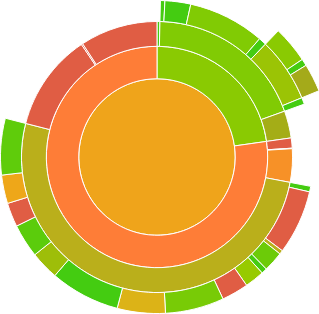
\includegraphics[width=.5\linewidth]{./starburst.png}
  \caption{Starburst representation of coinflip's current test coverage, primarily identify a lack of coverage for CLI functionality.}
\end{figure}

80.2\% of code is covered right now, with missing tests mainly residing in the CLI-related code files. This would be remedied by expanding the functionality of the CLI state machine (section \ref{sec:model}), and progress of which can be visually analysed by starburst charts over time.

\section{Evaluation}
\label{sec:orga7452af}
I believe the test strategy of coinflip covers is a good foundation, particularly in the potential of wholly comparing coinflip's randomness tests to other suites can establish coinflip as battle-tested---even if I myself have no real background in statistics or cryptography.

The Q3 aspect is only fulfilled by the exploratory nature of the Hypothesis library. A study with real users would be useful in the assessing coinflip's user experience by observing actual human behaviour.

\pagebreak
\begin{tabular}{ l r }
	Code repository: & \url{https://github.com/Honno/coinflip/} \\
	Documentation: & \url{https://coinflip.readthedocs.io/}\\
	Video demo: & \url{https://www.youtube.com/watch?v=0xrWG3Ki9Z8}\\
	& \small{(testing strategy begins at 11:39)}
\end{tabular}
\bibliographystyle{ieeetr}
\bibliography{refs}

\pagebreak
\appendix
\section{Sample of generated binary sequences}
\label{sec:sequences}
Sample of the consecutive binary sequences (represented per-line) run on coinflip's randomness tests.
\scriptsize{\begin{verbatim}
01
10
110
111100110001
010
01000
110
11001110
010
0101
100
0011011000001
0011011000001
0011011100001
0010011100001
0010011100001
0010011100001
0011011100001
1110101111
0011001
0011001
1011001
1011101
101
100
10100
00110101010
0110101010
0110101010
0110101010
0110101010
0110101010
011
1111001
1001
01
011110
011111
011111
000110
0001100
0001101
0001101
0001101
0011101
0001101
10010001111110100110
10010001111110110110
10010001111110110110
10010001011110110110
10010001011110110110
10010001011110110110
10010001011110111110
11001
1100
0100
001100
001100
000100
11101110101
011
111010010100
111010010101
111010010101
111010000101
11101000010110
1110100001011000110101110010
11000100111000
11000100111000
11000100011000
11000100011000
00001
01001
010
01011
0101110000
0101110000100
0101010000100
000011111110000
000011111110010
000011111110010
000011111111010
000010111111010
000010111111010
000010111111010
11110001111
11110101111
11110101111
11110101111
11110101111
11110100111
01110100111
01101100101001111
01101100101001111010010010011010
01101100101001111110010010011010
01101100101101111110010010011010
01101100101111111110010010011010
01101100101111111110010010011010
01101100101111111110010010011110
101
...and so on
\end{verbatim}}
\newpage
\section{Sample of generated CLI state machine runs}
\label{sec:stateful_example}
\scriptsize{\begin{verbatim}
>>> SETUP new state machine
    LOAD store1 with sequence 10
    TEARDOWN state machine
>>> SETUP new state machine
    TEARDOWN state machine
>>> SETUP new state machine
    LOAD store1 with sequence 10010
    LOAD store2 with sequence 11011
    REMOVE store1
    LS stores, check store1 not listed
    TEARDOWN state machine
>>> SETUP new state machine
    LOAD store1 with sequence 11111001010
    LOAD store2 with sequence 00101
    REMOVE store1
    LS stores, check store1 not listed
    REMOVE store2
    LS stores, check store2 not listed
    LOAD store3 with sequence 001111
    LS stores, check store3 listed
    LOAD store4 with sequence 011011000011001
    TEARDOWN state machine
>>> SETUP new state machine
    TEARDOWN state machine
>>> SETUP new state machine
    TEARDOWN state machine
>>> SETUP new state machine
    TEARDOWN state machine
>>> SETUP new state machine
    TEARDOWN state machine
>>> SETUP new state machine
    TEARDOWN state machine
>>> SETUP new state machine
    LOAD store1 with sequence 1000011001001000010
    LOAD store2 with sequence 001100010100
    LOAD store3 with sequence 111110111001
    LOAD store4 with sequence 1011101000110111
    LOAD store5 with sequence 1010
    LOAD store6 with sequence 0101101
    LOAD store7 with sequence 11111010001100
    TEARDOWN state machine
>>> SETUP new state machine
    TEARDOWN state machine
>>> SETUP new state machine
    LOAD store1 with sequence 11100
    LOAD store2 with sequence 10010
    LOAD store3 with sequence 1000011110
    LOAD store4 with sequence 01111
    REMOVE store1
    LS stores, check store1 not listed
    REMOVE store4
    LS stores, check store4 not listed
    LOAD store5 with sequence 01101010100000111
    TEARDOWN state machine
>>> SETUP new state machine
    LOAD store1 with sequence 011100100
    REMOVE store1
    LS stores, check store1 not listed
    LOAD store2 with sequence 1011100001
    LOAD store3 with sequence 000000111110
    REMOVE store2
    LS stores, check store2 not listed
    LOAD store4 with sequence 0000000010001101110010110010110101
    REMOVE store4
    LS stores, check store4 not listed
    TEARDOWN state machine
>>> SETUP new state machine
    TEARDOWN state machine
>>> SETUP new state machine
    TEARDOWN state machine
>>> SETUP new state machine
    LOAD store1 with sequence 11000111101101111011000
    LOAD store2 with sequence 11101011010101
    LS stores, check store1 listed
    LOAD store3 with sequence 1101
    LOAD store4 with sequence 011110110001011
    REMOVE store2
    LS stores, check store2 not listed
    LOAD store5 with sequence 1101001001010100
    LOAD store6 with sequence 11001011
    TEARDOWN state machine
>>> SETUP new state machine
    TEARDOWN state machine
>>> SETUP new state machine
    TEARDOWN state machine
>>> SETUP new state machine
    TEARDOWN state machine
>>> SETUP new state machine
    TEARDOWN state machine
>>> SETUP new state machine
    TEARDOWN state machine
>>> SETUP new state machine
    TEARDOWN state machine
>>> SETUP new state machine
    TEARDOWN state machine
>>> SETUP new state machine
    LOAD store1 with sequence 00101
    REMOVE store1
    LS stores, check store1 not listed
    LOAD store2 with sequence 10111000101001101100
    LOAD store3 with sequence 10011010000000100001011010
    REMOVE store3
    LS stores, check store3 not listed
    LOAD store4 with sequence 011
    LOAD store5 with sequence 11110100
    TEARDOWN state machine
    ...and so on
\end{verbatim}}

\end{document}